\documentclass{article}
\usepackage{listings}
\usepackage{mathrsfs}
\usepackage[utf8]{inputenc}
\usepackage{amssymb}
\usepackage{lipsum}
\usepackage{amsmath}
\usepackage{fancyhdr}
\usepackage{geometry}
\usepackage{scrextend}
\usepackage[english,german]{babel}
\usepackage{titling}
\setlength{\droptitle}{-3cm}
\usepackage{tikz}
\usepackage{algorithm,algpseudocode}
\usepackage[doublespacing]{setspace}
\usetikzlibrary{datavisualization}
\usetikzlibrary{datavisualization.formats.functions}
\usepackage{polynom}
\usepackage{amsmath}
\usepackage{gauss}
\usepackage{tkz-euclide}
\usetikzlibrary{datavisualization}
\usetikzlibrary{datavisualization.formats.functions}
\author{
Alexander Mattick Kennung: qi69dube\\
Kapitel 1
}
\usepackage{import}
\date{\today}
\geometry{a4paper, margin=2cm}
\usepackage{stackengine}
\parskip 1em
\newcommand\stackequal[2]{%
  \mathrel{\stackunder[2pt]{\stackon[4pt]{=}{$\scriptscriptstyle#1$}}{%
  $\scriptscriptstyle#2$}}
 }
\makeatletter
\renewcommand*\env@matrix[1][*\c@MaxMatrixCols c]{%
  \hskip -\arraycolsep
  \let\@ifnextchar\new@ifnextchar
  \array{#1}}
\makeatother
\lstset{
  language=haskell,
}
\lstnewenvironment{code}{\lstset{language=Haskell,basicstyle=\small}}{}
\usepackage{enumitem}
\setlist{nosep}
\usepackage{titlesec}
\usepackage{ stmaryrd }
\usepackage{verbatim}


\titlespacing*{\subsection}{0pt}{2pt}{3pt}
\titlespacing*{\section}{0pt}{0pt}{5pt}
\titlespacing*{\subsubsection}{0pt}{1pt}{2pt}
\title{Vorlesung 4}


\begin{document}
	\maketitle
	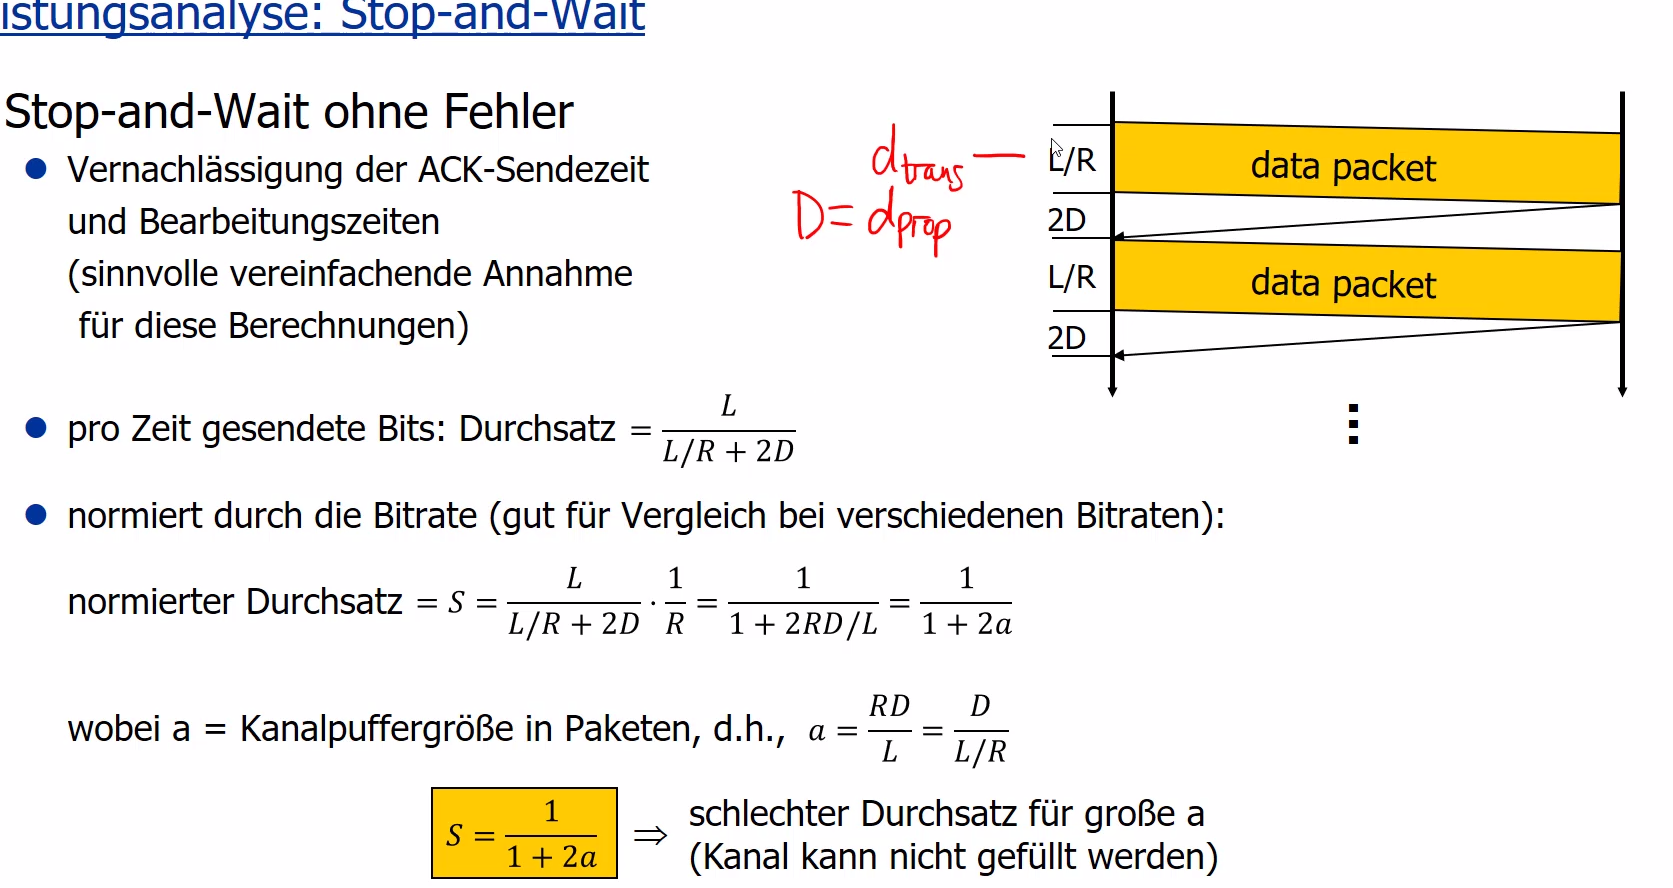
\includegraphics[width=256px]{Stop-And-Wait.png}\\
	je größer die Kanalpufferrate a, desto schlechter.\\
	$S[Auslastung]=\frac{1}{1+2a} = \frac{1}{1+2\frac{RD}{L}}$\\
	Wenn $O[Objektgroesse]=NL$ wenn man N erhöht, sinkt L, also nenner wird kleiner. Also schlechter Auslastung\\
	Wenn $O[Objektgroesse]=NL$ wenn man L erhöht, wird der Nenner größer. Bessere Auslastung\\
	(man muss seltener die 2d aufs ACK warten)\\
	Datenrate ist R=4,0kbps und Ausbreitungsverzögerung D=20ms.\\
	ges.: L\\
	$S=0.5 = \frac{1}{1+2\frac{RD}{L}} = \frac{1}{1+2\frac{4*0.020}{L}}$\\
	$2 = 1+2\frac{4*0.020}{L}$\\
	$1 = 2\frac{4*0.020}{L}$\\
	$2*4*0.020 = L$\\
	$2*4*0.020=160bit = L$\\
	also ab Paketgröße 160bit erhalten wir mit Stop-and-wait eine effizienz S=0.5\\
	Bei stop-and-wait (und konstantem Kanal...) reichen 2 SNR aus, weil sich immer max. ein Paket im Transit ist.\\
	Man benötigt kein NAK (ablehnen des Empfangs, bei z.B. fehler) im ALternating bit protokoll, da bei einem Fehler einfach das ACK des zuletzt erhalten pakets nochmal senden (bzw timeout durchlaufen lassen)\\
	Bei Schiebefenstern 2 Fälle:\\
	Fall 1 Fenster ist nicht groß genug, um Kanal auszulasten (also das Fenster lastet nicht 2D+L/R aus)\\
	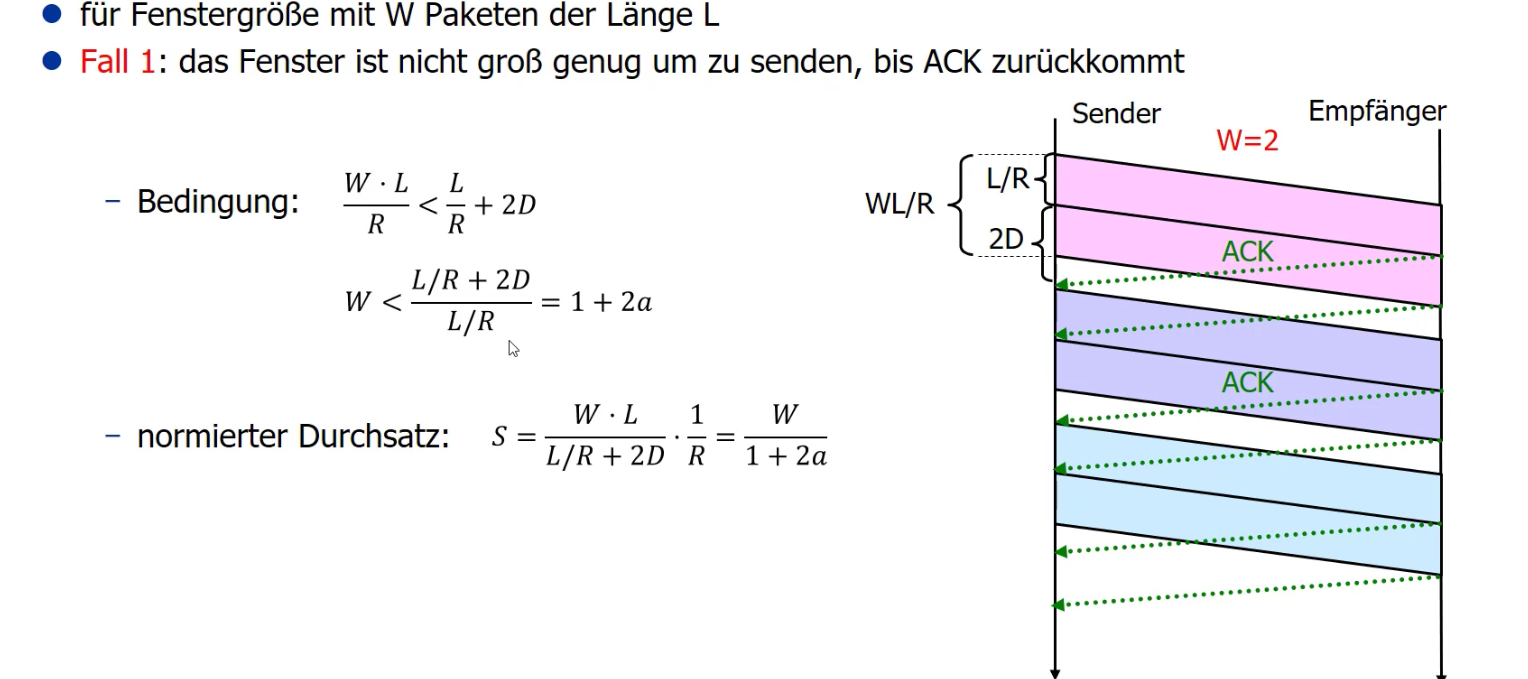
\includegraphics[width=256px]{GOBACKNsmallwindow.png}\\
	Im fall, dass das fenster groß genug ist, kann kontinuierlich gesendet werden (das ACK kommt vor ende des Schiebefensters an) perfekte auslastung:\\
	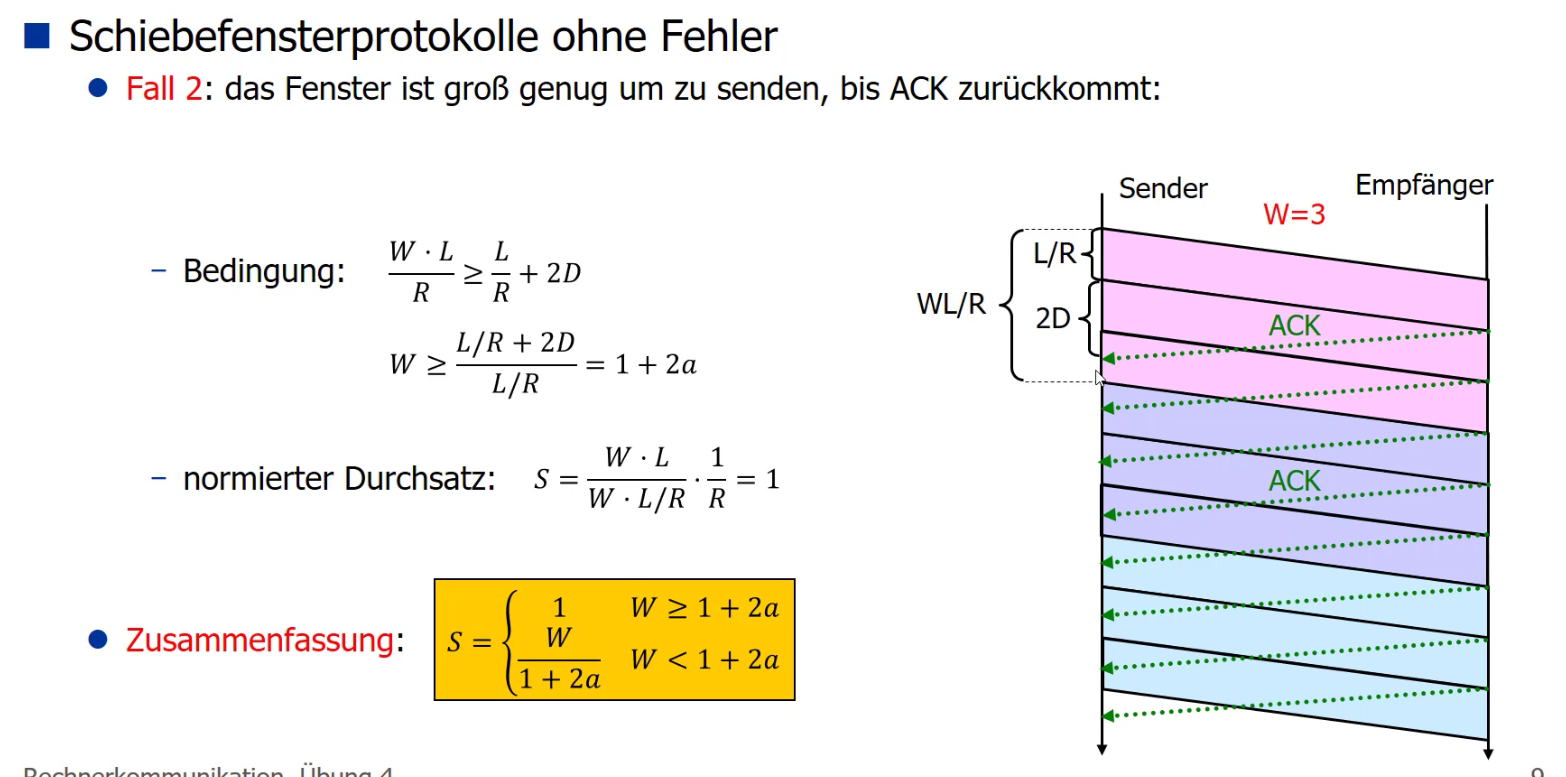
\includegraphics[width=256px]{GOBACKNlargeWindow.png}\\
	Übung 4.4\\
	Satelit mit 1,0Mbps=R 270ms=D L = 1000Bit.\\
	ges $S_1, S_7, S_{127},S_{255}$\\
	$\frac{W}{1+2\frac{RD}{L}} = \frac{W}{1+2\cdot 270Kb/1000bit} = \frac{W}{1+2*270}=\frac{W}{1+0.54} = \frac{W}{541}$\\
	W ist immer kleiner als $1+2a=541$ (also S nie = 1)\\
	$S_1 = \frac{1}{541} = 0.18\%$\\
	$S_7 = \frac{7}{541}= 1.3\%$\\
	$S_{127}= \frac{127}{541}= 23\%$\\
	$S_{255}= \frac{256}{541}=47\%$\\
	Übung 4.5\\
	geg.\\
	$R_{AB} = 1000\frac{kbit}{s}, d_{prop} = 10\mu s/km, L=1000bit, W_{AB} = 3, W_{BC}=1, l_{AB}=2000km, l_{BC} = 500km$\\
	ges $R_{BC}$ sodass es keinen Stau bei B gibt.\\
	Lsg.: Alles was in B reingeht, muss im selben moment wieder rauskommen, also muss der Durchsatz (NICHT der normierte) gleich sein.\\
	$S_{AB} R_{AB} = S_{BC}R_{BC}$ (also entnormieren)\\
	Zuerst testen was $1+2a$ und $1+2a<W$ überprüfen.\\
	$a_{ab} = \frac{100kbps*20ms}{1000bit} = 2\implies 1+2a = 5>3$\\
	$\frac{w_{AB}}{1+2a_{AB}}R_{AB}= \frac{1}{1+2a_{BC}}*R_{BC} $\\
	$\frac{3}{5}1000kbps= \frac{1}{1+2a_{BC}}*R_{BC}\implies R_{BC} = 150kbps$\\

\end{document}
